% Nallino, Part I p. 190: the analemma of al-Battānī's rule for the hour angle, redrawn from the print: the meridian
% AFPB as a half circle over the horizon AB; the horizon, the equator EC and the parallel FG as straight lines; the
% perpendiculars FL and HK and the axis from C to the pole in dashes, each where it printed; the bold italic letters
% and the word Polus. Measured on the scan (_intake/latin/tools/fig190).
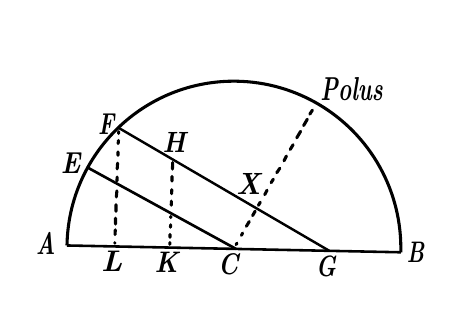
\begin{tikzpicture}[x=0.9928pt,y=-0.9928pt,line cap=butt,every node/.style={font=\fontsize{11}{11}\bfseries\itshape\selectfont,inner sep=0pt}]
\useasboundingbox (0,0) rectangle (147.00,94.00);
\draw[line width=0.93pt] (14.31,79.27) -- (135.80,81.75);  % the horizon AB
\draw[line width=0.96pt] (21.84,50.92) -- (75.84,80.53);  % the equator EC
\draw[line width=0.88pt] (32.99,36.40) -- (109.79,81.22);  % the parallel FG
\draw[line width=1.11pt] (14.31,79.28) arc[start angle=180.90,end angle=361.44,radius=60.76];
% the dashes of FL, of HK and of the axis from C to the pole
\draw[line width=1.11pt,line cap=round] (33.06,41.04)--(32.92,42.18) (32.87,45.20)--(32.87,46.44) (32.74,49.30)--(32.57,51.41) (32.47,59.40)--(32.26,61.63) (32.15,64.38)--(32.16,66.82) (31.96,69.31)--(31.98,71.51) (31.89,73.57)--(31.81,75.31) (33.13,37.85)--(33.10,38.53);
\draw[line width=1.11pt,line cap=round] (32.55,54.34)--(32.50,55.79) (31.71,78.22)--(31.71,78.44) (52.54,54.12)--(52.53,55.84) (52.45,58.96)--(52.40,60.45) (52.29,63.13)--(52.26,64.62) (52.04,71.73)--(51.96,72.64) (51.81,75.22)--(51.80,76.34) (52.77,49.08)--(52.69,51.49);
\draw[line width=1.11pt,line cap=round] (52.09,68.70)--(52.08,69.14) (51.76,78.22)--(51.74,78.86) (103.64,30.02)--(102.69,31.48) (101.78,33.31)--(100.44,35.64) (99.34,37.72)--(97.94,40.09) (96.61,42.60)--(95.55,44.34) (94.16,46.73)--(93.31,48.45) (91.78,51.16)--(90.66,52.79);
\draw[line width=1.11pt,line cap=round] (89.41,55.15)--(88.61,56.43) (87.13,59.16)--(86.29,60.77) (84.65,63.52)--(83.99,64.68) (80.65,70.56)--(79.59,72.30) (78.23,74.75)--(77.79,75.59) (76.17,78.44)--(75.86,78.95) (82.79,66.79)--(81.87,68.41);
\node at (117.91,22.14) {\normalfont\fontsize{11}{11}\bfseries\itshape\selectfont \resizebox{22.51pt}{8.32pt}{Polus}};
\node at (28.54,34.94) {\normalfont\fontsize{11}{11}\bfseries\itshape\selectfont \resizebox{5.83pt}{7.49pt}{F}};
\node at (53.25,41.68) {\normalfont\fontsize{11}{11}\bfseries\itshape\selectfont \resizebox{8.29pt}{7.26pt}{H}};
\node at (15.67,49.24) {\normalfont\fontsize{11}{11}\bfseries\itshape\selectfont \resizebox{7.05pt}{7.51pt}{E}};
\node at (80.33,56.76) {\normalfont\fontsize{11}{11}\bfseries\itshape\selectfont \resizebox{8.88pt}{7.61pt}{X}};
\node at (6.51,78.52) {\normalfont\fontsize{11}{11}\bfseries\itshape\selectfont \resizebox{7.07pt}{7.72pt}{A}};
\node at (141.19,81.60) {\normalfont\fontsize{11}{11}\bfseries\itshape\selectfont \resizebox{6.27pt}{7.36pt}{B}};
\node at (30.63,85.18) {\normalfont\fontsize{11}{11}\bfseries\itshape\selectfont \resizebox{7.68pt}{7.38pt}{L}};
\node at (50.51,85.54) {\normalfont\fontsize{11}{11}\bfseries\itshape\selectfont \resizebox{8.51pt}{7.36pt}{K}};
\node at (73.01,85.94) {\normalfont\fontsize{11}{11}\bfseries\itshape\selectfont \resizebox{7.31pt}{7.39pt}{C}};
\node at (108.56,87.08) {\normalfont\fontsize{11}{11}\bfseries\itshape\selectfont \resizebox{7.33pt}{7.28pt}{G}};
\end{tikzpicture}
